%%%%%%
%
% $Autor: Wings $
% $Datum: 2020-01-18 11:15:45Z $
% $Pfad: WuSt/Skript/Produktspezifikation/powerpoint/ImageProcessing.tex $
% $Version: 4620 $
%
%%%%%%

%Quelle: https://towardsdatascience.com/from-lenet-to-efficientnet-the-evolution-of-cnns-3a57eb34672f


%\begin{figure}[!h]
%    %\begin{subfigure}[h]{0.4\linewidth}
%%todo Eigene Bilder    
%    \includegraphics[width=0.7\textwidth]{CoralTPU/Concept/dogs}
%\end{figure}
% {\tiny Quelle: \href{https://machinelearners.net/2017/08/23/predicting-bitcoins-value-using-convolution-neural-networks-long-short-term-memory-cells/}{Vaibhav Sharma : Predicting bitcoin’s Value Using Convolution neural networks \& Long short term memory cells!} \cite{Sharma:2017}}



%todo 
%\url{https://machinelearners.net/2017/08/23/predicting-bitcoins-value-using-convolution-neural-networks-long-short-term-memory-cells/}



%Inspired n from the  program image classification on coral Usb accleator coded by Adrian, a similar procedure was followed to program this  image classification program .\newline
\section{Convolution Neural Network}

Ein Schwerpunkt für das Maschinelle Lernen liegt in der Interpretation von Bildern. Hier müssen zwei Fälle unterschieden werden

\begin{enumerate}
    \item Detektion von Objekten\index{Detektion von Objekten}
    \item Klassifikation von Bildern.\index{Klassifikation von Bildern}
    
\end{enumerate}. 

Bei der Detektion von Objekten wird ein Bild untersucht, ob ein oder mehrere Objekte identifiziert werden können. Falls ein Objekt erkannt wird, so werden die Koordinaten des umgebenden Rechtecks und die Klasse  oder die Klassen des Objekts mit einer jeweiligen Wahrscheinlichkeit zurückgeliefert. Bei der Segmentierung\index{Segmentierung} wird anstelle der Koordinaten des umgebenden Rechtecks ein Polygonzug zurückgeliefert, der das Objekt umgibt. Demgegenüber wird bei er Klassifizierung eines Bilder eine Beschreibung des Bildes gesucht. In beiden Fällen werden \ac{cnn} häufig eingesetzt, die in folgenden Abschnitt beschrieben werden. 

Ein \ac{cnn} erwartet als Eingabeinformation ein Bild. Wenn Bilder keine Farbinformationen enthalten werden sie als Matrizen dargestellt, deren Anzahl der Spalten und Reihen mit der Anzahl der Pixel in Breite und Höhe übereinstimmen. In dem Fall, dass ein Bild Farbinformationen enthält, so wird für jede Farbe eine solche Matrix angelegt. In diesem Fall spricht man von Farbkanal oder einfach nur von Kanal\index{Kanal}.


\ac{cnn} ist eine häufig verwendete shift-invariante Methode zur Extraktion von lernfähigen Merkmalen. Ihr Erfolg hat zur Popularität des Maschinellen Lernens beigetragen. In ihrer Historie haben ihre Architektur eine große Entwicklung vollzogen.\index{Alom:2018} Einige bekannte Architekturen werden nun beschrieben.    

\subsection{CNN-Architekturen}


\subsection{LeNet\index{LeNet}}

Die CNN-Architektur LeNet war 1998 die erste CNN-Architektur, die Back-Propagation für praktische Anwendungen nutzte. Damit transportierte sie Deep Learning von der Theorie in die Praxis. LeNet wurde für die Erkennung handgeschriebener Ziffern verwendet und konnte alle anderen bestehenden Methoden übertreffen. Die Architektur war mit nur 5 Schichten, bestehend aus $5\times 5$ Faltungen und $2 \times 2$ Max-Pooling, sehr einfach, ebnete aber den Weg zu besseren und komplexeren Modellen. \cite{LeCun:1998} Die Auflistung der Elemente in Tabelle~\ref{Concept:LeNet} enthält verschiedene Punkte, die später beschrieben werden.



% https://www.kaggle.com/blurredmachine/lenet-architecture-a-complete-guide


\begin{figure}
  \includegraphics[page=7,width=0.9\textwidth,viewport=20 600 560 740,clip]{../../MLbib/CNN/Lecun98.pdf}

  \caption{Struktur der CNN-Architektur gemäß LeCun et.al. \cite{LeCun:1998}}\label{Concept:LeNet}
\end{figure}

\begin{table}
  \begin{tabular}{ccc ccc c}
  	\multicolumn{2}{c}{\textbf{Layer}} & \textbf{\begin{tabular}{c}Feature\\ Map \end{tabular}} & \textbf{Größe} & \textbf{\begin{tabular}{c} Größe \\des\\ Kerns\\ \end{tabular}} & \textbf{Stride} & \textbf{\begin{tabular}{c}Akti- \\vierungs- \\funktion \end{tabular}}  \\ \hline
  	Eingabe  & Bild            &   1 & $32\times 32$ &            - & - & - \\
  	1        & Convolution     &   6 & $28\times 28$ &  $5\times 5$ & 1 & $\tanh$ \\  
  	2        & \begin{tabular}{c}Average\\ Pooling  \end{tabular} &   6 & $14\times 14$ &  $2\times 2$ & 2 & $\tanh$ \\  
  	3        & Convolution     &  16 & $10\times 10$ &  $5\times 5$ & 1 & $\tanh$ \\  
    4        & \begin{tabular}{c}Average\\ Pooling  \end{tabular} &  16 &   $5\times 5$ &  $2\times 2$ & 2 & $\tanh$ \\  
  	5        & Convolution     & 120 &   $1\times 1$ &  $5\times 5$ & 1 & $\tanh$ \\  
  	6        & \begin{tabular}{c}Neural\\ Network  \end{tabular} &   - &          $84$ &    -         & - & $\tanh$ \\  
  	Ausgabe  & \begin{tabular}{c}Neural\\ Network  \end{tabular}  &   - &          $10$ &    -         & - & softmax \\  
  \end{tabular}  		
  \caption{Strukturelememte von LeNet}
%  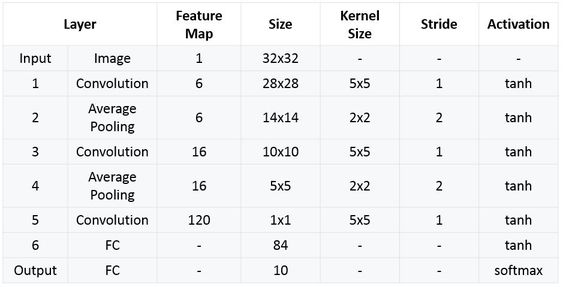
\includegraphics[scale=0.7]{Bilder/CNN/LeNetStructure}

\end{table}

  


\subsection{AlexNet\index{AlexNet}} 

Die Architektur AlexNet nutzte als erstes CNN-Modelle, das auf \ac{gpu}s implementiert wurde.  2012 wurde damit die wachsende Rechenleistung wirklich mit Deep Learning verbunden. AlexNet ist deutlich tiefer und komplexer als LeNet Sie fingen auch an, ReLU-Aktivierungen anstelle von Sigmoid oder tanh zu verwenden, was dazu beitrug, bessere Modelle zu trainieren. AlexNet gewann nicht nur den ImageNet-Klassifizierungswettbewerb 2012, sondern schlug den Zweitplatzierten mit einem Vorsprung, der nicht-neuronale Modelle plötzlich fast obsolet machte. \cite{Krizhevsky:2012}

%https://www.kaggle.com/blurredmachine/alexnet-architecture-a-complete-guide


\subsection{InceptionNet\index{InceptionNet}}


Die Architektur InceptionNet\index{InceptionNet} nutzte die gesteigerten Möglichkeiten der Hardware. Die Architektur war wieder deutlich tiefer und parameterreicher als die bestehenden Modelle. Um mit dem Problem des Trainings tieferer Modelle umzugehen, verwendeten sie die Idee mehrerer Hilfsklassifikatoren, die zwischen dem Modell vorhanden sind, um zu verhindern, dass der Gradient abbricht. Eine ihrer Ideen war die parallele Verwendung von Kerneln verschiedener Größen und damit die Erhöhung der Breite des Modells anstelle der Tiefe. Damit kann eine solche Architektur sowohl größere als auch kleinere Merkmale gleichzeitig zu extrahieren. \cite{Szegedy:2014}


\subsection{VGG\index{VGG}}

Viele Architekturen versuchten durch größere Faltungskerne bessere Ergebnisse zu erzielen. So wird bei der Architektur AlexNet\index{AlexNet} unter anderem Kerne der Größe $11 \times 11$ verwendet. Die Architektur VGG\index{VGG} wurde der Weg beschritten, mehrere Kerne der Größe $3\times 3$ hintereinander  und mehr Nichtlinearitäten in Form von Aktivierungsfunktionen zu verwenden. Damit konnten die Ergebnisse wieder verbessert werden. \cite{Zhang:2015,Simonyan:2015}

\subsection{Residual Neural Network (ResNet)\index{ResNet}}

% https://towardsdatascience.com/an-overview-of-resnet-and-its-variants-5281e2f56035
Je tiefer die Architekturen wurden, desto häufiger trat das Problem beim Training auf, dass der Betrag des Gradienten zu gering wurde. Die Backpropagation\index{Backpropagation} brach dann ab und die Parameter konnten nicht bestimmt werden. In der Architektur \ac{resnets} wurde zur Verhinderung des Problems Rest- oder Abkürzungsverbindungen eingeführt, die alternative Pfade für den Gradienten schaffen, um die mittleren Schichten zu überspringen und direkt die Anfangsschichten zu erreichen. Auf diese Weise konnten die Autoren extrem tiefe Modelle trainieren, die zuvor keine gute Leistung zeigten. Es ist mittlerweile gängige Praxis, in modernen CNN-Architekturen Restverbindungen zu haben. \cite{He:2016}




\subsection{MobileNet \& MobileNetV2\index{MobileNet}\index{MobileNetV2}} %: Moving towards edge-friendly models

Die Architektur MobileNet ist für Edge Computer und Smart Phones konzipiert, die im Bereich des Speichers und der Rechenleistung begrenzt sind. Damit konnte ein großes Feld neuer Anwendungen eröffnet werden. Im Gegensatz zur bisherigen Strategie, die Architekturen immer weiter zu vergrößern, in dem trennbare Faltungen eingeführt wurden. Vereinfacht ausgedrückt, wird ein zweidimensionaler Faltungskern in zwei separate Faltungen aufgeteilt, und zwar in die Tiefenfaltung, die für das Sammeln der räumlichen Informationen für jeden einzelnen Kanal zuständig ist, und in die Punktfaltung, die für die Interaktion zwischen den verschiedenen Kanälen verantwortlich ist. Später wurde auch MobileNetV2 mit Restverbindungen und anderen Optimierungen in der Architektur eingeführt, um die Modellgröße weiter zu reduzieren. \cite{Howard:2017,MobileNet:2018}

\subsection{EfficientNet\index{EfficientNet}} %: Squeeze and Excitation layers

Die Architektur ist das Ergebnis der Betrachtung, dass die bisherigen verschiedenen Architeklturen, sich entweder auf die Leistung oder die Recheneffizienz konzentrieren. Die Autoren von \cite{Tan:2020} behaupteten, dass diese beiden Probleme durch ähnliche Architekturen gelöst werden können. Sie schlugen eine gemeinsame CNN-Skelettarchitektur und drei Parameter vor, nämlich die Breite, die Tiefe und die Auflösung. Die Breite des Modells bezieht sich auf die Anzahl der Kanäle, die in den verschiedenen Schichten vorhanden sind, die Tiefe bezieht sich auf die Anzahl der Schichten im Modell und die Auflösung bezieht sich auf die Größe des Eingabebildes für das Modell. Sie behaupteten, dass man ein konkurrenzfähiges und dennoch rechnerisch effizientes CNN-Modell erstellen kann, wenn man alle diese Parameter klein hält. Auf der anderen Seite kann man durch Erhöhen des Wertes dieser Parameter ein Modell erstellen, das auf Genauigkeit ausgerichtet ist.

%
%Obwohl Squeeze- und Excitation-Schichten bereits früher vorgeschlagen wurden, waren sie die ersten, die diese Idee in Mainstream-CNNs einführten. S\& E-Schichten erzeugen kanalübergreifende Interaktionen, die invariant gegenüber räumlichen Informationen sind. Dies kann genutzt werden, um den Einfluss von weniger wichtigen Kanälen zu verringern. Sie führten auch die neu vorgeschlagene Swish-Aktivierung anstelle von ReLU ein, was ein wichtiger Faktor für die Leistungsverbesserung war. EfficientNets sind derzeit die leistungsstärksten Klassifikationsmodelle unter verschiedenen Kategorien der Verfügbarkeit von Rechenressourcen.

\subsection{Allgemeiner Aufbau}



In der Beschreibung der Architekturen wurden einige Elemente, die zum Aufbau notwendig sind, erwähnt. Alle Bausteine können wie folgt aufgelistet werden:

\begin{itemize}
  \item Faltungsschicht (Convolution)
  \item Aktivierungsfunktion
  \item Pooling
  \item Flatten
  \item Neuronales Netz
\end{itemize}

Jeder Baustein wird durch weitere Größen charakterisiert. Die Kombination und Konfiguration der Bauelemente werden in den sogenannten Hyperparameter zusammengefasst. Durch die Angabe der  Hyperparameter\index{Hyperparameter} ist die Architektur und die Anzahl der Parameter festgelegt. Beispielsweise bei einem neuronalen Netz sind die Hyperparameter\index{Hyperparameter} die Anzahl der Layer, die Anzahl der Neuronen je Layer und die Festlegung der Aktivierungsfunktionen. Werden nun die Anzahl aller Neuron bestimmt, so ergibt daraus die Anzahl der Parameter, die während des Trainings ermittelt werden

In der Tabelle~\ref{concept:Parameter} werden einige Architekturen verglichen. Die Tabelle gibt die Aznahl der Parameter an, die zu trainieren sind.  Falls ein Bild klassifiziert wird, so geben die Modelle verschiedene Möglichkeiten an und belegen diese mit einer Wahrscheinlichkeit. Die Genauigkeit gibt nun den Prozentsatz an, mit dem das Bild mit der Vorhersage mit der höchsten Wahrscheinlichkeit übereinstimmt. Dazu wurde die Modelle mit dem ImageNet\index{ImageNet} trainiert und validiert. 




 \begin{table}
   \begin{tabular}{lllrc}
     Modell            & Größe  & Genauigkeit & Parameter   & Tiefe \\ \hline
     VGG16             & 528 MB & 71{,}3\%    & 138.357.544 & 23 \\     
     VGG19             & 549 MB & 71{,}3\%    & 143.667.240 & 26 \\     
     ResNet-50         &  98 MB & 74{,}9\%    &  25.636.712 & 50 \\     
     ResNet-101        & 171 MB & 76{,}4\%    &  44.707.176 & 101 \\     
     ResNet-152        & 232 MB & 76{,}6\%    &  60.419.944 & 152 \\     
     InceptionV3       &  92 MB & 77{,}9\%    &  23,851,784 & 159 \\
     InceptionResNetV2 & 215 MB & 80{,}3\%    &  55,873,736 & 572 \\
%     NASNetMobile      &  23 MB & 74{,}4\%    &   5.326.716 & --\\
%     NASNetLarge       & 343 MB & 82{,}5\%    &  88.949.818 & --\\
     MobileNet         &  16 MB & 70,{4}\%    &   4.253.864 & 88 \\       
     MobileNetV2       &  14 MB & 71,{3}\%    &   3.538.984 & 88 \\       
    \end{tabular}
  \caption{Kenngrößen verschiedener \ac{cnn}-Architekturen\index{VGG}\index{ResNet}\index{Inception}\index{MonileNet}}\label{concept:Parameter}
 \end{table}
 
Die einzelnen Bausteine werden nun im Folgenden beschrieben.



\subsection{Ein- und Ausgabe}

Wenn ein Modell ein Bild als Eingabe bekommt, so werden Felder mit Pixelwerten übergeben. Die Höhe, die Breite und die Anzahl der Farbkanäle bestimmen die Größe der Felder. Die Elemente der Felder enthalten dann Werte zwischen Null und 255. Dieser Wert ist die Intensität des Pixels. Das Modell ermittel dann auf der Grundlage dieser Felder Wahrscheinlichkeiten, wie ein Bild zu klassifizieren ist. So könnte das Ergebnis sein, dass das Bild zu $81\%$ eine Schildkröte, zu $11\%$ eine Gewehr und zu $8\%$ eine Schokoladenriegel darstellt.


%todo Sichtbar machen der Filter, Lernen der Filter



\subsection{Faltungsschicht}\label{subsec:conv2d}

In einer Faltungsschicht, auch Convolution gnannt, werden die Eingangsdaten durch einen oder mehrere Filter modifiziert. Bei der Bildverarbeitung handelt es sich dabei um die Anwendung einer definierten Menge von Filtern auf zweidimensionale Daten.

Die Größe dieses Filters wird durch den sogenannten Kern definiert: ein $3 \times 3$-Kern wird durch eine $3 \times 3$-Matrix dargestellt. Um den Filter anwenden zu können, wird ein Bereich der Pixelwert festgelegt, der die gleiche Größe hat; die Pixelwerte werden dann auch in eine Matrix abgelegt. Durch die Faltung der Matrix, wie sie in der Gleichung~\ref{concept:FaltungMatrix} dargestellt ist, wird der Matrix und dem Filter ein wert zugeordnet. 
    
   
    \begin{figure}
        
        $$A \ast C 
        =
        \left(
        \begin{matrix}
            a_{11} & a_{12} & a_{13}\\
            a_{21} & a_{22} & a_{23}\\
            a_{31} & a_{32} & a_{33}\\
        \end{matrix}
        \right)
        \ast
        \left(
        \begin{matrix}
            c_{11} & c_{12} & c_{13}\\
            c_{21} & c_{22} & c_{23}\\
            c_{31} & c_{32} & c_{33}\\
        \end{matrix}
        \right)
        = 
        \sum_{i=1}^3\sum_{j=1}^3  a_{ij} \cdot c_{ij}
        $$
        
        \caption{Definition der Faltung zweier Matrizen}\label{concept:FaltungMatrix}
        
    \end{figure}
 
 Zur Anwendung eines Filters müssen also systematisch Matrizen aus den Pixelwerten ausgewählt werden. Da die Dimension eines Kerns durch eine ungerade Zahl $2n+1$ festgelegt ist, kann jedem Pixelwert, der einen Abstand größer als $n$ vom Rand hat eine umgebende Matrix zugeordnet werden. In der Abbildung~\ref{concept:conv2d} ist eine solche Situation dargestellt. Der Filter, mit $C$ bezeichnet und lila eingefärbt, hat eine Dimension von $3 \times 3$. In der Matrix $A$, dem Feld der Pixelwerte, ist ein Bereich rot eingefärbt. In der Mitte befindet sich der Pixel von der fünften Spalte und der zweiten Reihe. Auf diesen Bereich der Matrix $A$ wird nun der Filter angewendet. Das Ergebnis wird dann in die Matrix $A\ast C$ eingetragen. In diesem Fall ist der Wert $4$ und grün markiert.
 
  
 Ein Filter wird nun Schrittweise über die Daten bewegt.  Der Filter kann dabei auf jeden Pixelwert angewendet werden, der vom Rand weit genug entfernt ist, oder es können einzelne Pixel übersprungen werden. Dies wird durch die Schrittgröße, auch stride genannt, definiert. Bei einer Schrittgröße von Eins wird jeder Pixel verwendet. Um die Ausgabe Größe zu reduzieren, können auch Schrittgrößen größer als Eins verwendet werden; es ist auch möglich unterschiedliche Schrittgröße für die Breite und die Höhe festzulegen. Falls eine Schrittgröße von $2$ in beide Richtungen vorgegeben ist, so hat sich die Datenmenge auf $25\%$ reduziert. \cite{Dumoulin:2016}
 
 In der Abbildung~\ref{concept:conv2d} ist die Eingangsmatrix eine $7\times 7$-Matrix. Da hier eine Schrittgröße von Eins angewendet wird, ist das Ergebnis eine $5\times 5$-Matrix.
    
 Häufig wird auf jedes Ergebnis noch eine Aktivierungsfunktion angewendet.
    
    \begin{figure}[htb]
        
       
        \centering
        \begin{tikzpicture}
            % SOURCE: https://github.com/PetarV-/TikZ/blob/master/2D%20Convolution/2d_convolution.tex
            \matrix (mtr) [matrix of nodes,row sep=-\pgflinewidth, nodes={draw}]
            {
                0 & 1 & 1 & |[fill=red!20]| 1 & |[fill=red!20]| 0 & |[fill=red!20]| 0 & 0\\
                0 & 0 & 1 & |[fill=red!20]| 1 & |[fill=red!20]| 1 & |[fill=red!20]| 0 & 0\\
                0 & 0 & 0 & |[fill=red!20]| 1 & |[fill=red!20]| 1 & |[fill=red!20]| 1 & 0\\
                0 & 0 & 0 & 1 & 1 & 0 & 0\\
                0 & 0 & 1 & 1 & 0 & 0 & 0\\
                0 & 1 & 1 & 0 & 0 & 0 & 0\\
                1 & 1 & 0 & 0 & 0 & 0 & 0\\
            };
            
            \draw[very thick, red!20] (mtr-1-4.north west) rectangle (mtr-3-6.south east);
            
            \node [below= of mtr-5-4.south] (lm) {$\mathbf{A}$};
            
            \node[right = 0.2em of mtr] (str) {$*$};
            
            \node (ast2) at (2,-2) {$\mathbf{*}$};
            \node (ast2) at (4,-2) {$\mathbf{=}$};
            
            \matrix (K) [right=0.2em of str,matrix of nodes,row sep=-\pgflinewidth, nodes={draw, fill=blue!20}]
            {
                1 & 0 & 1 \\
                0 & 1 & 0 \\
                1 & 0 & 1 \\
            };
            \node [below = of K-3-2.south] (lk) {$\mathbf{C}$};
            
            \node [right = 0.2em of K] (eq) {$=$};
            
            \matrix (ret) [right=0.2em of eq,matrix of nodes,row sep=-\pgflinewidth, nodes={draw}]
            {
                1 & 4 & 3 & |[fill=green!20]| 4 & 1\\
                1 & 2 & 4 & 3 & 3\\
                1 & 2 & 3 & 4 & 1\\
                1 & 3 & 3 & 1 & 1\\
                3 & 3 & 1 & 1 & 0\\
            };
            \node [below = of ret-4-3.south] (lim) {$\mathbf{A} \ast  \mathbf{C}$};
            
            \draw[very thick, green!20] (ret-1-4.north west) rectangle (ret-1-4.south east);
            
            \draw[densely dotted, blue!30, thick] (mtr-1-4.north west) -- (K-1-1.north west);
            \draw[densely dotted, blue!30, thick] (mtr-3-4.south west) -- (K-3-1.south west);
            \draw[densely dotted, blue!30, thick] (mtr-1-6.north east) -- (K-1-3.north east);
            \draw[densely dotted, blue!30, thick] (mtr-3-6.south east) -- (K-3-3.south east);
            
            \draw[densely dotted, green!30, thick] (ret-1-4.north west) -- (K-1-1.north west);
            \draw[densely dotted, green!30, thick] (ret-1-4.south west) -- (K-3-1.south west);
            \draw[densely dotted, green!30, thick] (ret-1-4.north east) -- (K-1-3.north east);
            \draw[densely dotted, green!30, thick] (ret-1-4.south east) -- (K-3-3.south east);
            
            \matrix (K) [right=0.2em of str,matrix of nodes,row sep=-\pgflinewidth, nodes={draw, fill=blue!20}]
            {
                1 & 0 & 1 \\
                0 & 1 & 0 \\
                1 & 0 & 1 \\
            };
            
            \draw[very thick, blue!20] (K-1-1.north west) rectangle (K-3-3.south east);
            
            \node[anchor=south east, inner sep=0.01em, blue!20] at (mtr-1-4.south east) (xx) {\scalebox{.5}{$\times 1$}};
            \node[anchor=south east, inner sep=0.01em, blue!20] at (mtr-1-5.south east) (xx) {\scalebox{.5}{$\times 0$}};
            \node[anchor=south east, inner sep=0.01em, blue!20] at (mtr-1-6.south east) (xx) {\scalebox{.5}{$\times 1$}};
            \node[anchor=south east, inner sep=0.01em, blue!20] at (mtr-2-4.south east) (xx) {\scalebox{.5}{$\times 0$}};
            \node[anchor=south east, inner sep=0.01em, blue!20] at (mtr-2-5.south east) (xx) {\scalebox{.5}{$\times 1$}};
            \node[anchor=south east, inner sep=0.01em, blue!20] at (mtr-2-6.south east) (xx) {\scalebox{.5}{$\times 0$}};
            \node[anchor=south east, inner sep=0.01em, blue!20] at (mtr-3-4.south east) (xx) {\scalebox{.5}{$\times 1$}};
            \node[anchor=south east, inner sep=0.01em, blue!20] at (mtr-3-5.south east) (xx) {\scalebox{.5}{$\times 0$}};
            \node[anchor=south east, inner sep=0.01em, blue!20] at (mtr-3-6.south east) (xx) {\scalebox{.5}{$\times 1$}};	
        \end{tikzpicture}
        \caption{Faltungsschicht mit $3 \times 3$ Kern und Schrittgröße (1, 1)}
        \label{concept:conv2d}
        
    \end{figure}
    
Bei der Definition der Filter ist darauf zu achten, dass für jeden Kanal der Filter definiert ist.
Um die Merkmale in einem Bild zu erfassen, müssen die Werte in dem Filter mit der Struktur der ursprünglichen Pixelwerten des Bildes übereinstimmen. Grundsätzlich gilt, wenn im Eingangsbild eine Form vorhanden ist, die im Allgemeinen der Kurve ähnelt, welche dieser Filter darstellt, dann ergibt sich aus der Faltung ein großer Wert.

In der Regel werden mehrere Filter parallel eingesetzt. Das Ergebnis sind sogenannte Feature Maps\index{Feature Maps}. Auf dieses Ergebnis werden dann weitere Faltungsschichten  angewendet, die wiederum Feature Maps generieren. 


\subsubsection{Merkmal-Identifikation}

Eine Faltung wird durch Filter definiert. Jeder Filter kann als Identifikator von Merkmalen interpretiert werden. Merkmale sind zum Beispiel Kanten, Farben oder auch Kurven. Beispielsweise wird der $7\times 7$-Filter betrachtet:

$$\left(
\begin{array}{ccc ccc c}
    0 & 0 & 0 &  0 & 0  & 50 & 0 \\
    0 & 0 & 0 &  0 & 50 &  0 & 0 \\
    0 & 0 & 0 & 50 &  0 &  0 & 0 \\
    0 & 0 & 0 & 50 &  0 &  0 & 0 \\
    0 & 0 & 0 & 50 &  0 &  0 & 0 \\
    0 & 0 & 0 & 50 &  0 &  0 & 0 \\
    0 & 0 & 0 &  0 &  0 &  0 & 0 \\
\end{array}
\right)
$$  

Dieser Filter kann auch als Bilder visualisiert werden:

%todo Image generieren



Um die Wirkung des Filters zu demonstrieren, wird ein Beispielbild~\ref{concept:FilterCat} betrachtet:


\begin{figure}
  \centering    

%todo Eigenes Bild
  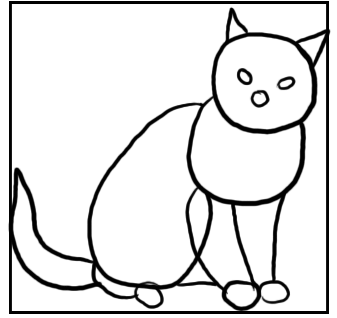
\includegraphics[scale=0.3]{CNN/cat}
    
  \caption{Beispielanwendung für einen Filter und ein Ausschnitt}\label{concept:FilterCat}
\end{figure}

In dem Beispielbild~\ref{concept:FilterCat} ist ein Ausschnitt markiert, auf den der Filter anwendet wird. 



$$
\left(
\begin{array}{ccc ccc c}
    0 & 0 & 0 &  0 & 0  &  0 & 30 \\
    0 & 0 & 0 &  0 & 80 & 80 & 80 \\
    0 & 0 & 0 & 30 & 80 &  0 &  0 \\
    0 & 0 & 0 & 80 & 80 &  0 &  0 \\
    0 & 0 & 0 & 80 & 80 &  0 &  0 \\
    0 & 0 & 0 & 80 & 80 &  0 &  0 \\
    0 & 0 & 0 & 80 & 80 &  0 &  0 \\
\end{array}
\right)
\star
\left(
\begin{array}{ccc ccc c}
    0 & 0 & 0 &  0 & 0  & 50 & 0 \\
    0 & 0 & 0 &  0 & 50 &  0 & 0 \\
    0 & 0 & 0 & 50 &  0 &  0 & 0 \\
    0 & 0 & 0 & 50 &  0 &  0 & 0 \\
    0 & 0 & 0 & 50 &  0 &  0 & 0 \\
    0 & 0 & 0 & 50 &  0 &  0 & 0 \\
    0 & 0 & 0 &  0 &  0 &  0 & 0 \\
\end{array}
\right)$$

$$
=
\left(
\begin{array}{ccc ccc c}
    0 & 0 & 0 &  0 & 0  &  0 & 30 \\
    0 & 0 & 0 &  0 & 80 & 80 & 80 \\
    0 & 0 & 0 & 30 & 80 &  0 &  0 \\
    0 & 0 & 0 & 80 & 80 &  0 &  0 \\
    0 & 0 & 0 & 80 & 80 &  0 &  0 \\
    0 & 0 & 0 & 80 & 80 &  0 &  0 \\
    0 & 0 & 0 & 80 & 80 &  0 &  0 \\
\end{array}
\right)
$$  

Es wird die grundsätzliche Eigenschaft von Filter verdeutlicht. Wenn im Eingabebild eine Form vorhanden ist, die im Allgemeinen dem Filter ähnelt, dann ergeben große Werte. Über die Aktivierungsfunktion wird dann eine Wahrscheinlichkeit zugeordnet. In der Faltungsschicht werden dann verschiedene Filter definiert und angewendet. Das Ergebnis ist dann die Feature Map. In der Abbildung~\ref{concept:FilterVis} sind einige Beispiele für konkrete Visualisierungen von Filtern der ersten Faltungsschicht eines trainierten Netzwerks zu sehen. 


\begin{figure}[!h]
  \centering
    %\begin{subfigure}[h]{0.4\linewidth}
%  \includegraphics[width=0.7\textwidth]{CoralTPU/Concept/FirstLayers}
  
  \includegraphics[viewport=0 350 280 480,clip,page=2,width=0.7\textwidth]{../../MLbib/CNN/08663285.pdf}
    
  \caption{Visualisierung von Filtern eines trainierten Netzes \cite{Lu:2019,Shang:2016}}\label{concept:FilterVis}
\end{figure}


\subsubsection{Kantenerkennung}

Auch für eine Kantenerkennung können geeignete Filter definiert werden. Der Filter


$$\left(
\begin{array}{ccc}
    1 & 0 & -1 \\
    1 & 0 & -1 \\
    1 & 0 & -1 \\
\end{array}
\right)
$$

kann für einer vertikale Kantenerkennung verwendet werden, dagegen kann der Filter 


$$\left(
\begin{array}{ccc}
    1 &  1 &  1 \\
    0 &  0 &  0 \\
    -1 & -1 & -1 \\
\end{array}
\right)
$$

für eine horizontale genutzt werden. Beide Filter werden nun auf eine vertikale Kante angewendet.


\begin{figure}
$$
\left(
\begin{array}{ccc ccc}
    10 & 10 & 10 & 0 & 0 & 0 \\
    10 & 10 & 10 & 0 & 0 & 0 \\
    10 & 10 & 10 & 0 & 0 & 0 \\
    10 & 10 & 10 & 0 & 0 & 0 \\
    10 & 10 & 10 & 0 & 0 & 0 \\
    10 & 10 & 10 & 0 & 0 & 0 \\
\end{array}
\right)
\ast
\left(
\begin{array}{ccc}
    1 & 0 & -1 \\
    1 & 0 & -1 \\
    1 & 0 & -1 \\
\end{array}
\right)
=
\left(
\begin{array}{cccc}
    0 & 30 & 30 & 0 \\
    0 & 30 & 30 & 0 \\
    0 & 30 & 30 & 0 \\
    0 & 30 & 30 & 0 \\
\end{array}
\right)
$$

$$
\left(
\begin{array}{ccc ccc}
    10 & 10 & 10 & 0 & 0 & 0 \\
    10 & 10 & 10 & 0 & 0 & 0 \\
    10 & 10 & 10 & 0 & 0 & 0 \\
    10 & 10 & 10 & 0 & 0 & 0 \\
    10 & 10 & 10 & 0 & 0 & 0 \\
    10 & 10 & 10 & 0 & 0 & 0 \\
\end{array}
\right)
\ast
\left(
\begin{array}{ccc}
    1 &  1 &  1 \\
    0 &  0 &  0 \\
    -1 & -1 & -1 \\
\end{array}
\right)
=
\left(
\begin{array}{cccc}
    0 & 0 & 0 & 0 \\
    0 & 0 & 0 & 0 \\
    0 & 0 & 0 & 0 \\
    0 & 0 & 0 & 0 \\
\end{array}
\right)
$$
  \caption{Detektion von vertikalen und horizontalen Kanten}
\end{figure}

Kanten können in jeder beliebigen Anordnung in Bildern vorhanden sein, muss bei der Kantendetektion dies berücksichtigt werden. Das heißt, falls ein \ac{cnn} trainiert wird, so entwickeln sich die Filter anhand der vorgegebenen Bilder. 



\subsection{Padding}

In der bisherigen Darstellung konnten Filter nicht auf Randwerte angewendet werden. Einerseits werden dadurch Informationen nicht verwendet, andererseits reduziert sich die Größe der Bilder bei jeder Anwendung der Faltung. Um dies zu verhindern, wird das Padding angewendet. Bei einem Filter der Dimension $(2n+1) \times (2m+1)$, wird das Eingangsbild mit einem zusätzlichen Rand der Größe
$n$ und $m$. Die zusätzlichen Werte sind jeweils Null besetzt.



\subsection{Aktivierungsfunktion}\label{subsec:activation}

Die Aktivierungsfunktion wird auf den jeweiligen Ausgang einer Schicht angewandt und bestimmt durch Anwendung einer definierten Funktion, wie der Ausgangswert interpretiert werden soll. Hierbei werden die jeweiligen Eingangswerte, sowie einen Bias in die Berechnung mit einbezogen, und bestimmt, ob das Neuron ausgelöst wird \cite{Nwankpa:2018}. In diesem Beispiel wird dafür die \ac{relu}-Funktion angewandt: bei Eingangswerten kleiner gleich Null gibt die Funktion Null zurück, bei positiven Werten verhält sie sich linear \cite{Agarap:2018}. Es werden also ausschließlich positive Werte zurückgegeben (\cref{fig:relu}).

\begin{figure}
    \centering
    \begin{tikzpicture}
        \begin{axis}[
            domain=-5:5,
            axis equal,
            xmin=-5,
            xmax=5,
            axis y line=middle,
            axis x line=center,
            axis line style={->},
            xlabel={$x$},
            ylabel={$y$},
            xtick={-5,...,5},
            ytick={0,...,5},]
            \addplot+[mark=none,red,domain=-5:0] {0};
            \addplot+[mark=none,red,domain=0:5] {x};
        \end{axis}
    \end{tikzpicture}
    \caption{Darstellung der ReLu Aktivierungsfunktion}
    \label{fig:relu}
\end{figure}

Zum Beispiel kann nach einer Faltung eine Aktivierungsfunktion angewendet werden. Dies ist in der Gleichung~\ref{concept:AktivierungMatrix} dargestellt.


    \begin{figure}
    
    $$
      \ReLU(A) 
      = 
      \left(
        \begin{matrix}
          \ReLU(a_{11}+b) & \ReLU(a_{12} & \ldots & \ReLU(a_{1m}+b)\\
          \ReLU(a_{21}+b) & \ReLU(a_{22} & \ldots & \ReLU(a_{2m}+b)\\
             \vdots       & \ddots       &        &   \vdots \\
          \ReLU(a_{n1}+b) & \ReLU(a_{n2} & \ldots & \ReLU(a_{nm}+b)\\
    \end{matrix}
    \right)
    $$
    
    \caption{Anwendung einer Aktivierungsfunktion mit eines Bias $b \in \R$ auf eine Matrix}\label{concept:AktivierungMatrix}
    
\end{figure}





\subsection{Pooling}


Nach der Verwendung von Faltungsschichten werden bei \ac{cnn} häufig Pooling-Schichten eingesetzt, um die Größe der Darstellung zu reduzieren, um ebenso auch die Berechnungen zu beschleunigen sowie als auch einige der Erkennungsfunktionen etwas robuster machen. Dabei wird in der Regel zwischen zwei Pooling-Methoden unterschieden.

\begin{itemize}
  \item Max-Pooling
  \item Average-Pooling
\end{itemize}

Beim Pooling werden Bereiche einer Matrix zusammengefasst. Die Bereiche werden über zwei werte $n$ und $m$ definiert. Die Bereich sind Teilmatrizen der Matrix der Größe $n \times m$. Auf jede Untermatrix wird dann eine Funktion angewendet.

Beim Max-Pooling wird der maximale Wert der Untermatrix ermittelt und als Ergebnis eingetragen. Beim Average-Pooling wird statt des maximalen Werts der Durchschnittswert der Matrixelemente ermittelt und weiter verwendet.


Im Falle des Poolings wird ein Fenster mit einer definierten Größe über die Eingangsmatrix bewegt und der entsprechende Wert innerhalb des Fensters als zusammengefasster Wert übernommen. Die Schrittgröße, mit der das Fenster sich über die Matrix bewegt, wird über einen Parameter definiert \cite{Dumoulin:2016}. Der Standardwert entspricht der Größe der Untermatrix. Ein Beispiel ist in der Darstellung~\ref{fig:maxpooling2d} dargestellt: eine \twod{4}{4}-Matrix wird mit Größe \PYTHON{pool\_size}  \twod{2}{2} und einer Schrittweite \PYTHON{stride\_size} \twod{2}{2} verarbeitet. Da jeweils zwei Werte in jede Dimension zusammengefasst werden, halbieren sich die Dimensionen der Ausgangsmatrix im Gegensatz zur Eingangsmatrix. \cite{Britz:2015}

\begin{figure}[htb]
    \centering
    
    \def\yspacing{.75em}
    \begin{tikzpicture}[auto, node distance=0cm,>=latex']
        % Root folder blocks
        % Subfolder Blocks
        \node [smallblock] (bin) {2};
        \node [smallblock, below=of bin] (bin2) {0};
        \node [smallblock, right=of bin] (bin3) {0};
        \node [smallblock, right=of bin2] (bin4) {1};
        
        \node [smallblock, fill=blue!20, right=of bin3] (bin5) {1};
        \node [smallblock, fill=blue!20, below=of bin5] (bin6) {0};
        \node [smallblock, fill=blue!20, right=of bin5] (bin7) {1};
        \node [smallblock, fill=blue!20, right=of bin6] (bin8) {0};
        
        \node [smallblock, fill=green!20, below=of bin2] (bin9) {0};
        \node [smallblock, fill=green!20, below=of bin9] (bin10) {0};
        \node [smallblock, fill=green!20, right=of bin9] (bin11) {0};
        \node [smallblock, fill=green!20, right=of bin10] (bin12) {3};
        
        \node [smallblock, fill=yellow!20, right=of bin11] (bin13) {1};
        \node [smallblock, fill=yellow!20, below=of bin13] (bin14) {0};
        \node [smallblock, fill=yellow!20, right=of bin13] (bin15) {0};
        \node [smallblock, fill=yellow!20, right=of bin14] (bin16) {0};
        
        \node [smallblock, right=of bin8.east, xshift=10em] (res1) {2};
        \node [smallblock, fill=green!20, below=of res1] (res2) {3};
        \node [smallblock, fill=blue!20, right=of res1] (res3) {1};
        \node [smallblock, fill=yellow!20, right=of res2] (res4) {1};
        
        \draw [arrow] (bin8.south east)++(1em, 0) -- ($(res1.south west)+(-1em,0)$) node[midway, sloped, above] {\footnotesize pool\_size = (2,2)} node[midway, sloped, below] {\footnotesize stride = (2,2)};
    \end{tikzpicture}

    \bigskip
    
    \def\yspacing{.75em}
  \begin{tikzpicture}[auto, node distance=0cm,>=latex']
    % Root folder blocks
    % Subfolder Blocks
    \node [smallblock] (bin) {2};
    \node [smallblock, below=of bin] (bin2) {0};
    \node [smallblock, right=of bin] (bin3) {0};
    \node [smallblock, right=of bin2] (bin4) {1};
    
    \node [smallblock, fill=blue!20, right=of bin3] (bin5) {1};
    \node [smallblock, fill=blue!20, below=of bin5] (bin6) {0};
    \node [smallblock, fill=blue!20, right=of bin5] (bin7) {1};
    \node [smallblock, fill=blue!20, right=of bin6] (bin8) {0};
    
    \node [smallblock, fill=green!20, below=of bin2] (bin9) {0};
    \node [smallblock, fill=green!20, below=of bin9] (bin10) {0};
    \node [smallblock, fill=green!20, right=of bin9] (bin11) {0};
    \node [smallblock, fill=green!20, right=of bin10] (bin12) {3};
    
    \node [smallblock, fill=yellow!20, right=of bin11] (bin13) {1};
    \node [smallblock, fill=yellow!20, below=of bin13] (bin14) {0};
    \node [smallblock, fill=yellow!20, right=of bin13] (bin15) {0};
    \node [smallblock, fill=yellow!20, right=of bin14] (bin16) {0};
    
    \node [smallblock, right=of bin8.east, xshift=10em] (res1) {0{,}75};
    \node [smallblock, fill=green!20, below=of res1] (res2) {0{,}50};
    \node [smallblock, fill=blue!20, right=of res1] (res3) {0{,}75};
    \node [smallblock, fill=yellow!20, right=of res2] (res4) {0{,}25};
    
    \draw [arrow] (bin8.south east)++(1em, 0) -- ($(res1.south west)+(-1em,0)$) node[midway, sloped, above] {\footnotesize pool\_size = (2,2)} node[midway, sloped, below] {\footnotesize stride = (2,2)};
  \end{tikzpicture}

    \caption{Anwendung von Max-Pooling und Average-Pooling}
    \label{fig:maxpooling2d}
    
\end{figure}



%SubMatrix(A,i,j,k,l) = (a_{i,j})_{kl}
%\PYTHON{Max-Pooling(A, pool\_size, stride): $\R^{n \times n} \times \N^{2\times 2} \times \N^{2\times 2} \rightarrow \R^{m \times m}, 
%(A, (k_1,k_2), (m_1,m_2)) \mapsto  (\max( ))
%$$


\subsection{Flatten}\label{subsec:flatten}

Mit einem Flatten-Schicht wird das multidimensionale Eingangsobjekt in einen Vektor umgewandelt. Wenn beispielsweise ein Objekt mit den Dimensionen \threed{5}{7}{7} übergeben wird, resultiert daraus ein eindimensionaler Vektor mit 245 Elementen. In der Abbildung~\ref{fig:flatten} wird auf eine $3 \times 3$-Matrix die Funktion Flatten angewendet. Die Funktion kommt dann zum Einsatz, wenn nachfolgend ein neuronales Netz verwendet wird.

\begin{figure}[htb]
    \centering
    
    \def\yspacing{.75em}
    \begin{tikzpicture}[auto, node distance=0cm,>=latex']
        % Root folder blocks
        % Subfolder Blocks
        \node [smallblock] (bin) {1};
        \node [smallblock, right=of bin] (bin2) {1};
        \node [smallblock, right=of bin2] (bin3) {0};
        
        \node [smallblock, fill=blue!20, below=of bin] (bin3) {4};
        \node [smallblock, fill=blue!20, right=of bin3] (bin4) {2};
        \node [smallblock, fill=blue!20, right=of bin4] (bin5) {1};
        
        \node [smallblock, fill=green!20, below=of bin3] (bin6) {0};
        \node [smallblock, fill=green!20, right=of bin6] (bin7) {2};
        \node [smallblock, fill=green!20, right=of bin7] (bin8) {1};
        
        \node [smallblock, right=of bin5, xshift=6em] (res1) {1};
        \node [smallblock, right=of res1] (res2) {1};
        \node [smallblock, right=of res2] (res3) {0};
        \node [smallblock, fill=blue!20, right=of res3] (res4) {4};
        \node [smallblock, fill=blue!20, right=of res4] (res5) {2};
        \node [smallblock, fill=blue!20, right=of res5] (res6) {1};
        \node [smallblock, fill=green!20, right=of res6] (res7) {0};
        \node [smallblock, fill=green!20, right=of res7] (res8) {2};
        \node [smallblock, fill=green!20, right=of res8] (res9) {1};
        
        \draw [arrow] (bin5.east)++(1em, 0) -- ($(res1.west)+(-1em,0)$);
    \end{tikzpicture}
    \caption{Anwendung von Flatten}
    \label{fig:flatten}
    
\end{figure}

\subsection{Dense-Schicht}\label{subsec:dense}

In einer Schicht, oder auch Fully-Connected-Layer, handelt es sich um eine Schicht, die ein neuronales Netz verwendet. Dies bedeutet, dass jeder der vorherigen Ausgänge in jeden der Eingänge der Schicht gespeist werden. Ebenso wird jeder Ausgang mit jedem der folgenden Eingänge verknüpft. Diese Art von Schicht wird in der Regel dazu genutzt, um mit den durch die Faltung erzeugten Feature Maps eine Klassifizierung vornehmen zu können.  \cite{Keras:2020b} Sie wird durch die Anzahl der Neuronen und der zugehörigen Aktivierungsfunktion festgelegt.



\subsection{Verwendetes Modell bei einer CIFAR-10-Klassifizierung}\label{sec:usedmodel}

Bei dem verwendeten Modell handelt es sich um ein Objekt \mytt{keras.models.Sequential}. Mithilfe der Methode \mytt{add} können zu diesem Model die einzelnen Schichten   hinzugefügt. Der Aufbau des Modells ist dem Tensorflow-Tutorial für \acp{cnn} nachempfunden \cite{GoogleTensorFlowCNN:2020}. Die Struktur des Modells ist in \cref{fig:networklayers} abgebildet.

Die zuvor beschriebenen Schichten werden nun verwendet, um ein Modell zur Klassifizierung des  Datensatzes \ac{cifar}-10 mit Keras zu erstellen. Hierbei wird betrachtet, wie diese Schichten in der Python-Umgebung angewandt werden und wie sich die Größe und Dimension der Daten zwischen den einzelnen Schichten verändert. Die Dimensionen der Eingangs- sowie Ausgangsdaten der einzelnen Schichten sind in \cref{fig:networklayers} abgebildet.

\begin{code}
   \begin{lstlisting}[language=MyPython, numbers=left]
    MODEL = models.Sequential()
    MODEL.add(layers.Conv2D(filters=32, kernel_size=(3, 3), activation='relu', input_shape=(32, 32, 3)))
    MODEL.add(layers.MaxPooling2D(pool_size=(2, 2)))
    MODEL.add(layers.Conv2D(filters=64, kernel_size=(3, 3), activation='relu'))
    MODEL.add(layers.MaxPooling2D(pool_size=(2, 2)))
    MODEL.add(layers.Conv2D(filters=64, kernel_size=(3, 3), activation='relu'))
    MODEL.add(layers.Flatten())
    MODEL.add(layers.Dense(units=64, activation='relu'))
    MODEL.add(layers.Dense(units=10))
\end{lstlisting}
  \caption{Aufbau eines \ac{cnn} mit Keras}\label={src:cifarlayers}
\end{code}  

Zu Beginn wird, wie in \cref{sec:generatemodel} beschrieben, ein Keras-Objekt \PYTHON{Sequential} erzeugt. Die erste Schicht, die diesem Modell hinzugefügt wird, ist eine Faltungsschicht \PYTHON{Conv2D}, siehe Zeile 2. Dieser wird mit 32 Filtern mit einer Größe von jeweils \twod{3}{3} definiert. Wenn bei der Erstellung des Objekts der Parameter \mytt{stride} nicht explizit angegeben wird, wird auf die Standardschrittgröße (1, 1) zurückgegriffen. Da es sich bei den Eingangsdaten in das Modell um RGB-Bilder mit $32 \times 32$ Pixel  handelt, siehe \cref{sec:dataset}, wird als \PYTHON{input\_shape} \threed{32}{32}{3} angegeben. Durch diese Konfiguration werden die Eingangsdaten in der ersten Faltungsschicht von \threed{32}{32}{3} auf eine Ausgangsgröße von \threed{30}{30}{32} transformiert. Für jeden der angewandten Filter wird eine separate Feature Map hinterlegt.

Die nächste Schicht, eine Max-Pooling-Schicht mit einer \PYTHON{pool\_size} von \twod{2}{2}, reduziert die Datenmenge von \threed{30}{30}{32} auf \threed{15}{15}{32} (Zeile 3).

\begin{figure}[htb]
    \centering
    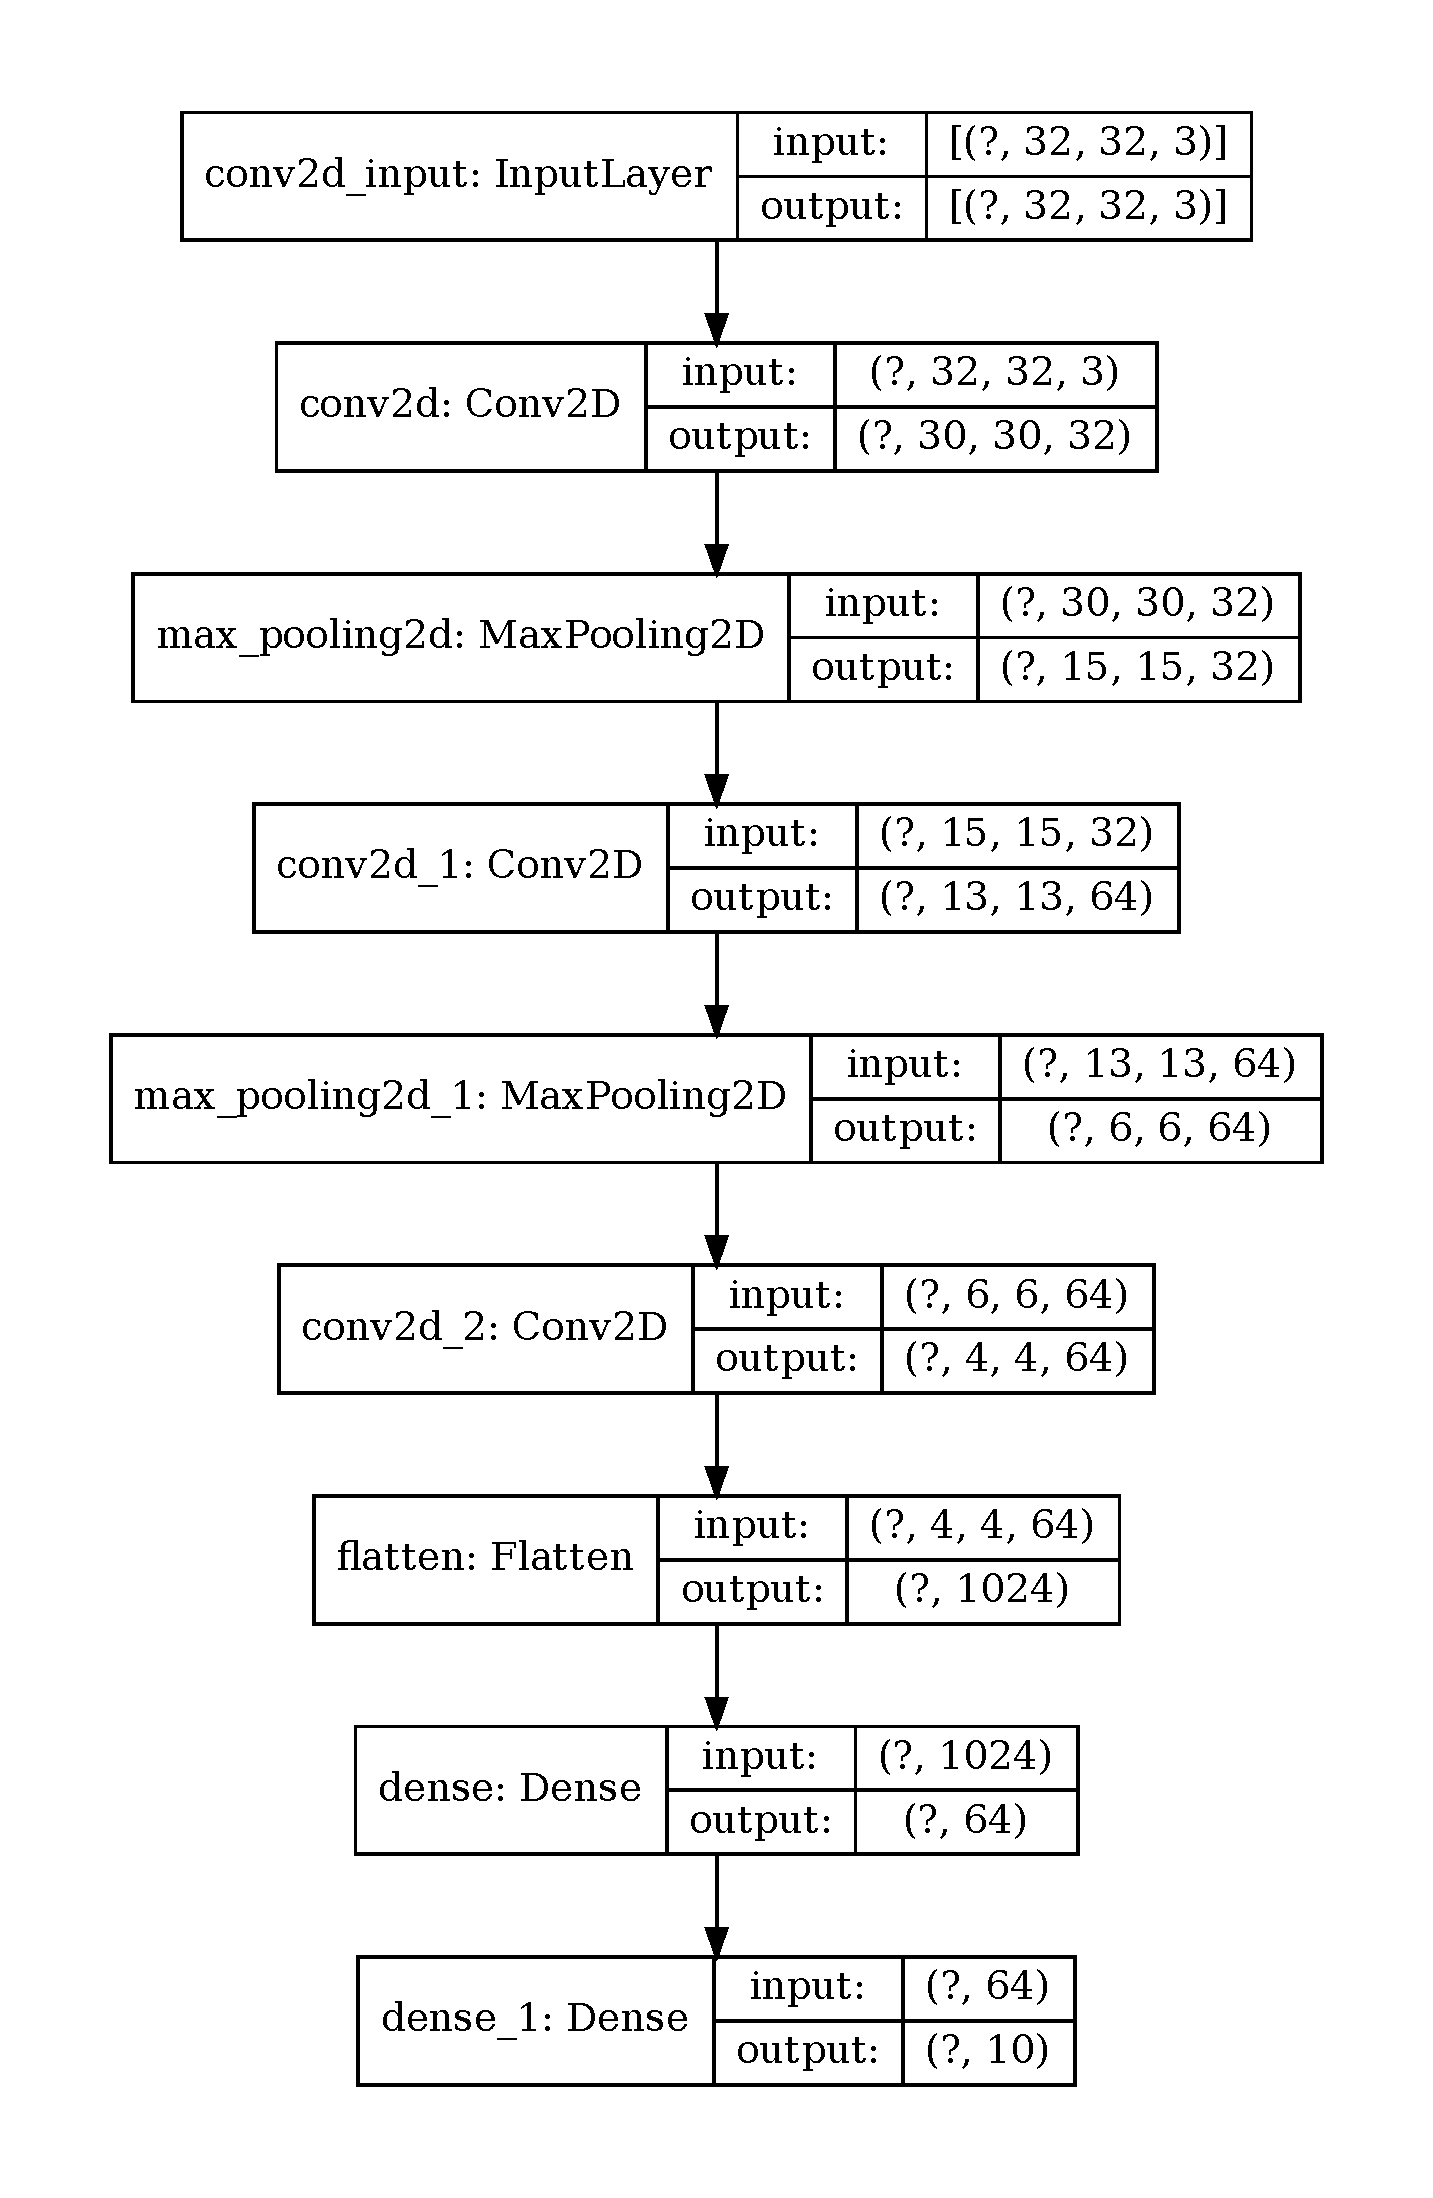
\includegraphics[trim = 0mm 19mm 0mm 19mm, clip, height=9cm]{Bilder/CUDA/cifar-model-graph-detailed.pdf}
    \caption{Aufbau des verwendeten neuronalen Netzes}
    \label{fig:networklayers}
\end{figure}

Diese Daten werden nun erneut in eine Faltungsschicht hineingegeben, welcher hier ebenfalls mit einer \PYTHON{kernel\_size} von \twod{2}{2}, \cref{src:cifarlayers}, Zeile 4, jedoch mit 64 Filtern konfiguriert wird. Dies transformiert die Daten von \threed{15}{15}{32} auf \threed{13}{13}{64}.

Um die Datenmenge erneut zu reduzieren, wird eine weitere Max-Pooling-Schicht angewandt, welcher ebenfalls mit einer \PYTHON{pool\_size} von \twod{2}{2}  in Zeile 5 konfiguriert wird  und somit die Datenmenge von \threed{13}{13}{64} auf \threed{6}{6}{64} verringert.

Im Anschluss wird der in diesem Netz die letzte Faltungsschicht angewandt. Diese arbeitet, wie die vorherige Faltungsschicht, mit \PYTHON{kernel\_size} \twod{2}{2} und 64 Filtern gemäß Zeile 6. Hierdurch werden die Daten von \threed{6}{6}{64} zu \threed{4}{4}{64} transformiert.

Um eine Klassifizierung dieser Informationen mit einem neuronalen Netz, der sogenannten Dense-Schicht, zu ermöglichen, werden die Ergebnisse der Faltungsschichten mit einer Flatten-Schicht in einen  Vektor transformiert, siehe Zeile 7. Durch die Eingangsgröße von \threed{4}{4}{64} resultiert dies in einen Vektor der Länge 1024.

Der Vektor wird in Zeile 8 in eine Dense-Schicht gespeist. Diese Schicht wird mit 64 \PYTHON{units} und der  Aktivierungsfunktion \ac{relu} parametrisiert, wodurch die 1024 Eingangsdaten in 64 Knoten zusammengefasst und die entsprechenden Ausgänge berechnet werden.

In der letzten Schicht werden die 64 Ausgangswerte in eine weiteren Dense-Schicht übergeben, welcher mit 10 \PYTHON{units} konfiguriert wurde. Die Eingangsdaten werden nun also auf 10 Ausgangsdaten reduziert, welche den zu identifizierenden Klassen des  Datensatzes \ac{cifar}-10 entsprechen.
 












